\documentclass[12pt,twoside]{report}

\usepackage[arrowdel]{physics}
\usepackage{siunitx}
\usepackage{amsmath}
\usepackage{amssymb}
\usepackage[margin=0.75in]{geometry}
\usepackage[margin=0.5in]{caption}
\usepackage[style=numeric-comp,backend=biber]{biblatex}
\usepackage[noblocks]{authblk}
\usepackage{graphicx}
\usepackage{subcaption}
\usepackage{tikz}
\usepackage{mhchem}
\usepackage{tipa}
\usepackage[hidelinks]{hyperref}
\usepackage{cleveref}

\setlength{\marginparwidth}{2cm}

\usetikzlibrary{patterns}

\addbibresource{biblio.bib}

\renewcommand\Affilfont{\small}
\newcommand*\mean[1]{\bar{#1}}

%% For the Hindmarsh-Rose model
\newcommand*{\hrx}{x}
\newcommand*{\hry}{y}
\newcommand*{\hrz}{z}
\newcommand*{\hra}{\alpha}
\newcommand*{\hrb}{\beta}

%% For the chimera-like index
\newcommand*{\chimera}{\chi}
\newcommand*{\meta}{m}
\newcommand*{\ordparam}{r}
\newcommand*{\phase}{\phi}

\author[1,2,5]{Henry Mitchell}
\author[1,4,5]{Peter Dodds}
\author[3,4]{Matt Mahoney}
\author[1,4,5]{Chris Danforth}
\affil[1]{Department of Mathematics and Statistics, University of Vermont College of Engineering and Mathematical Sciences}
\affil[2]{Department of Physics, University of Vermont College of Arts and Sciences}
\affil[3]{Department of Neurology, University of Vermont Larner College of Medicince}
\affil[4]{Department of Computer Science, University of Vermont College of Engineering and Mathematical Sciences}
\affil[5]{Computational Story Lab, Vermont Complex Systems Center, University of Vermont}

\title{Chimera States and Seizures in a Mouse Neuronal Model}

\begin{document}
\pagenumbering{alph}
\maketitle

\pagenumbering{arabic}

\begin{abstract}
  Mathematicians have observed the coexistence of synchronized and incoherent groups in coupled oscillator networks, known as ``chimera states.''
Recently, these models have been brought into theoretical neuroscience, where researchers are observing chimera states in simulations of animals' brains.
Many qualitative analogies have been drawn between chimera states collapsing into states of total synchrony and epileptic seizures, but quantitative evidence is lacking.
The goal of this project is to implement a coupled oscillator model on the human brain connectivity network, find the parameters of the model leading to chimera states, and observe whether their collapse matches data collected from human seizures.
%%% Local Variables:
%%% mode: latex
%%% TeX-engine: xetex
%%% TeX-master: "../main"
%%% End:

\end{abstract}

\tableofcontents

\chapter{Introduction}
\label{chap:intro}
As this work is an analysis of the relationship between chimera states and seizures, it is important to develop a baseline understanding of what each of those are.
\section{Chimera States}
\label{sec:intro_chimera}
\todo{Italicize terms.}
We show the normalized chimera-like index of the entire physical region in \cref{fig:aphysical_chimera}.
Near the maximal edge of the physical region, the highest values of the chimera index appear to follow a slope of $-1$.
It is unsurprising that chimera states would be prevalent when the coupling is large (out near the boundary of the aphysical range).

What is surprising, however, is the presence of the chimeric patch in the bottom left corner of \cref{fig:aphysical_chimera}, shown at a higher resolution in \cref{fig:zoom}.
\begin{figure}[ht]
  \centering
  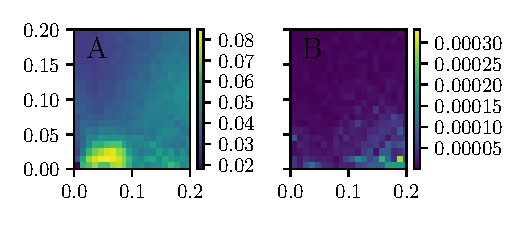
\includegraphics[width=0.5\textwidth]{figure/zoom_100dpi.pdf}
  \caption[Zoomed landscape]{A.\ The chimera-like index $\chimera$ of runs with $(\hra, \hrb) \in (0, 0.2) \times (0, 0.2)$.
    As before, the chimera-like index is normalized to $\frac{1}{7}$.
    Note that the values of the index are much higher in this patch than in most of the rest of $(\hra, \hrb) \in (0, 1) \times (0, 1)$ (\cref{fig:aphysical_chimera}).
    B.\ The variance of the chimera-like index.
  }
  \label{fig:zoom}
\end{figure}
Plotting the results of the simulations (\cref{fig:041_021}),
it is evident that this is not a calculation error, but is an actual feature of the parameter landscape.
\begin{figure*}[ht]
  \centering
  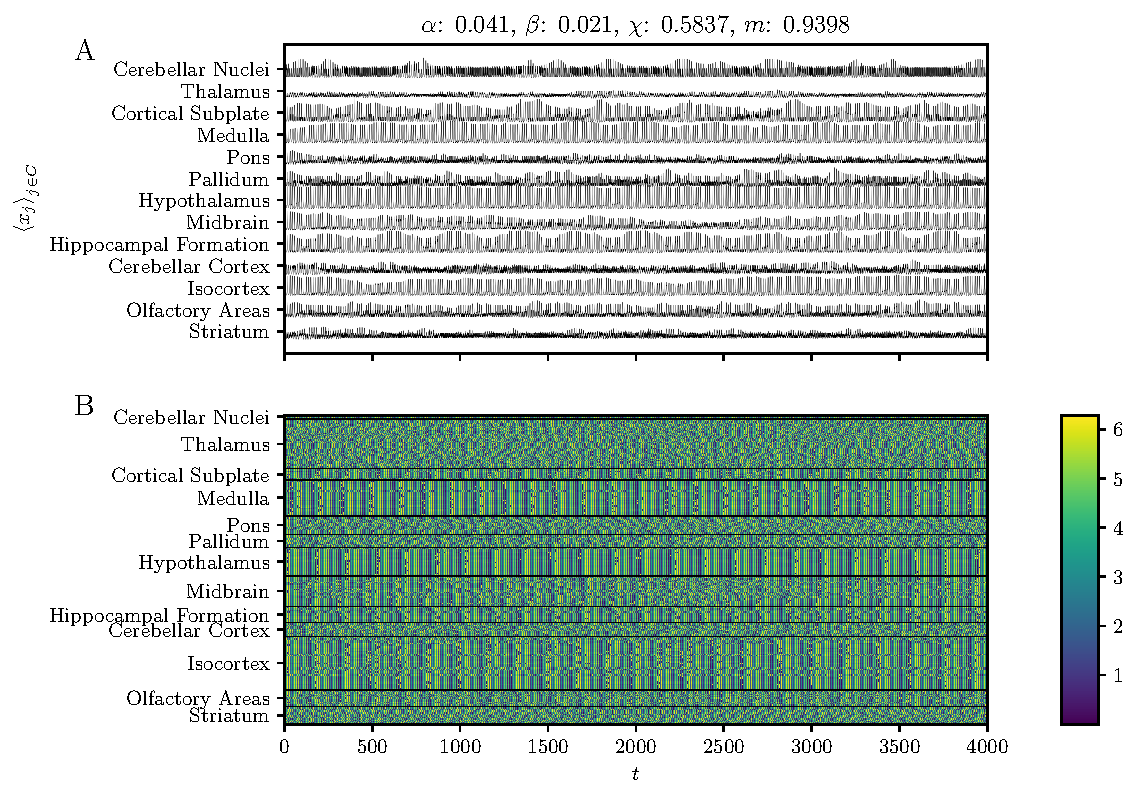
\includegraphics[width=\textwidth]{figure/0_041-0_021_200dpi.pdf}
  \caption[Highly chimeric simulation]{A run of the Hindmarsh-Rose simulation in the chimeric island.
    A. The mean membrane potential within each cortex.
    B. The phase $\phase$ of the entire timeseries for a simulation of the Hindmarsh-Rose network.
    Synchronization is most consistently evident in the medulla, the hypothalamus, and the isocortex.
  }
  \label{fig:041_021}
\end{figure*}

The highly chimeric patch within the physical portion of the landscape appears to be mostly below the $\beta = \alpha$ line.
This is reasonable, as chimera states occur when coupling within groups is greater than coupling between groups.
A small portion of the chimeric patch lies above the $\beta = \alpha$ line, likely because the average strength between cortices is greater than the average strength within cortices (see \cref{fig:average_strengths} A).

The chimera-like index $\chimera$ greatly lessens at $\alpha \approx 0.1$.
A possible explanation for this comes from comparing the order of $\dot{\hrx}$ without the coupling terms, and the coupling terms themselves.
From our simulation, we find that $\dot{\hrx}$ without the coupling terms ranges roughly from -6 to 3.
The coupling terms each\footnote{Since the same can be said for both $\alpha$ and $\beta$, we will discuss only $\alpha$, with the understanding that $\beta$ could be substituted into the proceeding sentences.}
range from 0 to approximately $30 \alpha$.
This means that, when $\alpha > 0.1$, the coupling is at least of the same order as the sum of the rest of the terms in the equation.
This leads to a qualitative difference between the two states, which likely manifests itself as the less-chimeric states.

%%% Local Variables:
%%% mode: latex
%%% TeX-master: "../../ms"
%%% End:


\section{Seizures}
\label{sec:intro_seizures}
\subsection{Neuroanatomy and Neurophysiology}
\label{sec:intro_seizures_neuroanatomy}
Since the brain is an electrochemical device, its function and disorders are often best talked about from an electrical standpoint \cite{Deco2008}.
\textit{Neurons} are cells which are specialized for communication (see \cref{fig:neuron_diagram} for a diagram).
\begin{figure}[ht]
  \centering
  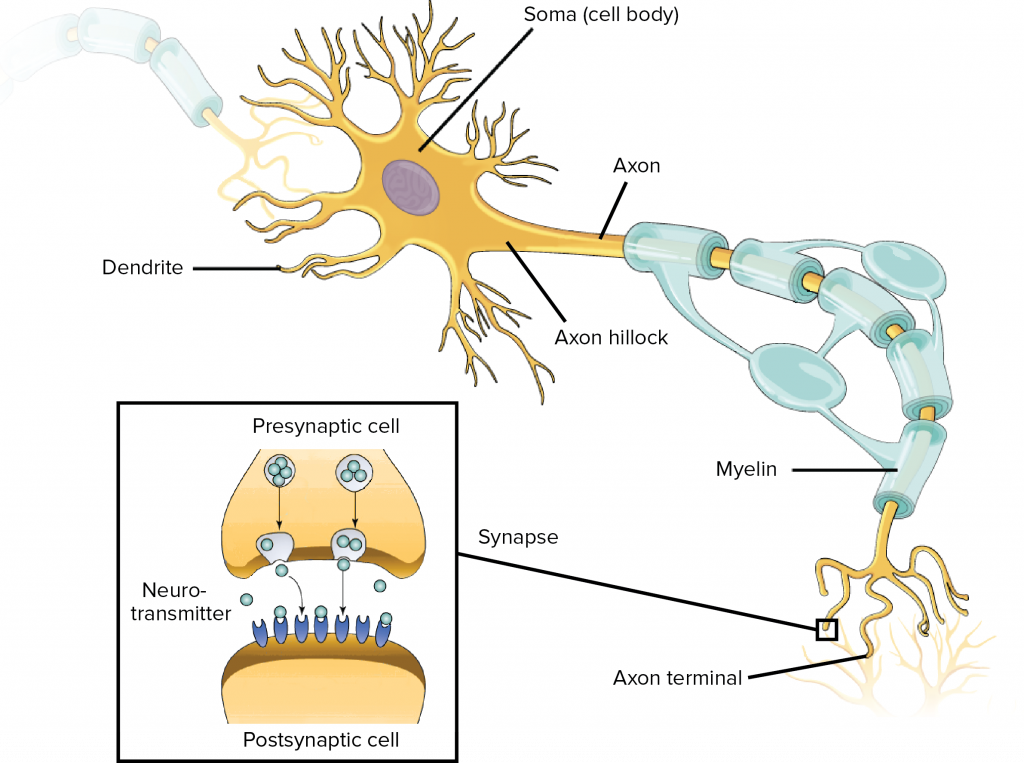
\includegraphics[width=0.5\textwidth]{figure/neuron_diagram}
  \caption[Neuron diagram]{A diagram of the anatomy of a neuron.
    Taken from \cite{Molnar2013}.
  }
  \label{fig:neuron_diagram}
\end{figure}
They receive input signals through \textit{synapses} at the ends of their \textit{dendrites}, branches in their large tree of inputs.
The trunk of the dendritic tree is the \textit{soma}, the cell body.
If the sum signal entering the soma from all of the dendrites is sufficient, the neuron \textit{fires}, sending a signal to its outputs.

When a neuron fires, it sends an electrochemical signal down its \textit{axon}---its long stem---to the output synapses at its \textit{axon terminals}.
This signal is known as an \textit{action potential}.
The action potential is discrete; a neuron sends the same signal any time its input threshold is surpassed, no matter how far above the threshold the input is.
It is the propagation along the axon of a potential difference across the cell membrane of the neuron.
This potential difference is created by different concentrations of various ions in and out of the cell, controlled by pumps (which push \ce{Na^{+}} out of the cell and draw \ce{K^{+}} into it) and gates (which allow the ion concentrations to equilibrate).
It is important to note that processes involving \ce{Na^{+}} are faster than those involving \ce{K^{+}}.
Each location along the axon goes through the following six stages, in total taking approximately \SI{1}{\ms}:
\begin{description}
\item[Equilibrium] No current flows through the membrane, which has a potential of \SI{-75}{\mV} across it\footnote{All potentials hold the extracellular matrix at \SI{0}{\V}.  In other words, the interior of the cell is at a lower potential than the exterior.}.

\item[Depolarization] The potential difference propagating from upstream in the axon activates ion channel gates, allowing \ce{Na^{+}} to flow into the axon, countered by the \ce{K^{+}} flowing out.

\item[Amplification] Because the \ce{K^{+}} processes are slower than the \ce{Na^{+}} processes, if the incoming signal is strong enough, the influx of \ce{Na^{+}} is too fast for the outflow of \ce{K^{+}} to compensate.
  This results in a positive feedback loop, wherein the \ce{Na^{+}} flowing in increases the membrane potential, which increases the rate at which \ce{Na^{+}} flows into the neuron, which continues to feed itself.

\item[Repolarization] When the \ce{Na^{+}} channels are fully open, the \ce{K^{+}} channels are finally able to compensate for the influx.

\item[Hyper-polarization] The \ce{Na^{+}} channels close, and the slower \ce{K^{+}} channels remain open.
  This causes more \ce{K^{+}} to flow out of the cell than \ce{Na^{+}} flowed in, dropping the potential below its equilibrium state.

\item[Refractory Period] The \ce{Na^{+}} channels are briefly unable to open, which means that neurons need a brief time to ``recharge'' after an action potential.

\end{description}

\subsubsection{Micro-scale models}
\label{sec:intro_seizures_neuroanatomy_hodgkin_huxley}
All of these processes are summarized in the \textit{Hodgkin-Huxley model}\footnote{A full derivation of this model can be found in \cite{Graben2008}.} describing the membrane potential $U$:
\begin{equation}
  \label{eq:hodgkin_huxley_main}
  C_{m} \dot{U}
  +
  p_{A \ce{K^{+}}} \mean{g}_{A \ce{K^{+}}} \pqty{U - E_{\ce{K^{+}}}}
  +
  p_{A \ce{Na^{+}}} \mean{g}_{A \ce{Na^{+}}} \pqty{U - E_{\ce{Na^{+}}}}
  +
  g_{l} \pqty{U - E_{l}}
  =
  I_{m}
\end{equation}
where
\begin{equation}
  \label{eq:hodgkin_huxley_supplementary}
  \begin{aligned}
    \dot{n}
    &=
    \alpha_{n} \pqty{1 - n} \beta_{n} n \\
    \dot{m}
    &=
    \alpha_{m} \pqty{1 - m} \beta_{m} m \\
    \dot{h}
    &=
    \alpha_{h} \pqty{1 - h} \beta_{h} h
  \end{aligned}
  \qand
  \begin{aligned}
    p_{A \ce{K^{+}}}
    &=
    n^{4} \\
    p_{A \ce{Na^{+}}}
    &=
    m^{3} h
  \end{aligned}
\end{equation}
where $g_{i}$ is the conductance of the membrane to ion $i$, $p_{A i}$ is the proportion of $i$-gates which are open (developed from a Markov model with transition rates $\alpha$ and $\beta$), $E_{i}$ is the equilibrium potential of ion $i$, $C_{m}$ is the capacitance of the membrane, and $I_{m}$ is an external current (the tuned input parameter).
This model is highly accurate, and won its developers a Nobel Prize in Physiology or Medicine.
Many bifurcation analyses have been performed on these equations, and they are well understood \cite{Graben2008}.

However, the Hodgkin-Huxley model is not particularly useful for large-scale brain simulation.
Given that most behavior of the brain is emergent\footnote{One of the classic ways to explain emergence is asking, ``Where is the thought in a neuron?''}, it is important to understand neurons' interactions.
As is often the case with emergent phenomena, it is wildly impractical to simulate the collective behavior of a brain by simulating its constituent neurons.
Since the human brain has approximately $10^{11}$ neurons with $10^{14}$ synapses, direct simulation is too computationally intensive.
In order to better understand the dynamics of large portions of the brain, many researchers turned to the techniques of thermal and statistical physics \cite{Breakspear2017}.
Particularly, \textit{neural ensemble models} and \textit{neural mass models} are popular approaches to studying brain behavior.

\subsubsection{Meso-scale Models}
\label{sec:intro_seizures_neuroanatomy_meso_scale}
Neural ensemble models treat patches of the brain as a collective group, taking into account neurons' mean activity, as well as their variance.
They assume that the firings of the neurons within a group are sufficiently uncorrelated to result in a Gaussian distribution of firing rates.
This means that the behavior of the ensemble is linear, even though the behavior of the constituent neurons is highly nonlinear.
One can then use a Fokker-Planck equation to describe the collective dynamics of the population.
The main benefit to these models is that they are well-studied in fields like solid-state physics.
However, recent work has shown that the assumption of Gaussian firing rates is not accurate \cite{Breakspear2017}.
Firing rates do tend to fall into well-behaved distributions, but not ones that lend themselves to already-developed tools.

For higher coherence within populations (i.e., a non-Gaussian distribution of firing rates), researchers tend to use neural mass models.
They assume that nearby neurons in the brain are sufficiently synchronized to model groups of them as a single neuron, with some modifications.
Instead of the discrete action potential of a single neuron, neural mass models often have a sigmoidal activation function.
They will also simplify the dynamics of the Hodgkin-Huxley model to divide the neural mass's constituent neurons into two subpopulations: an excitatory pool (corresponding to the \ce{Na^{+}} channels in the Hodgkin-Huxley model) and an inhibitory pool (corresponding to the \ce{K^{+}} channels in the Hodgkin-Huxley model).

An example of a neural mass model is the extremely simple Wilson-Cowan model \cite{Wang2012}:
\begin{align}
  \label{eq:wc_x}
  \tau_{x} \dot{x}
  &=
    -x + S \pqty{C_{x x} x + C_{x y} y + C_{x z} z + P} \\
  \label{eq:wc_y}
  \tau_{y} \dot{y}
  &=
    -y + S \pqty{C_{y x} x + C_{y y} y + C_{y z} z + Q} \\
  \label{eq:wc_z}
  \tau_{z} \dot{z}
  &=
    -z + S \pqty{C_{z x} x + C_{z y} y + C_{z z} z + R}
\end{align}
$x$ represents an excitatory process (like the flow of \ce{Na^{+}}), and $y$ and $z$ represent inhibitory processes (like the flow of \ce{K^{+}}).
The time constants $\tau_{i}$ determine the rates of the dynamics of the three processes.
It is worth noting that chaotic dynamics can occur when multiple different time scales are present \cite{Breakspear2017}.
The coupling strengths $C_{i j}$ represent the connectivity between the three processes, with $C_{i x} \geq 0$ (making $x$ excitatory) and $C_{i \Bqty{y, z}} \leq 0$ (making $y$ inhibitory).
$P$, $Q$, and $R$ represent the excitability threshold, or the constant external inputs to each process (similar to $I_{m}$ in \cref{eq:hodgkin_huxley_main}).
The sigmoidal activation function $S(x) = \frac{1}{1 + e^{-a \pqty{x - \theta}}}$ represents the mass effect of the population of neurons being modeled.
This system provides an excellent toy model which reflects meso-scale dynamics accurately, relative to its simplicity.

\subsubsection{Macro-scale Models}
\label{sec:intro_seizures_neuroanatomy_macro_scale}
These models do an accurate job of representing the behavior of small parts of the brain.
However, it is not reasonable to carry the assumptions of un- or highly-correlated activity to the large-scale activity of whole-brain dynamics.
In order to make these models accurately depict the overall behavior of the brain as a whole, researchers turn to two main techniques: \textit{neural field models} and \textit{neural mass networks}.
The first treats the brain as a continuous sheet of cortex, within which activity obeys wave equations.
The second represents the brain as a discrete graph of cortices, or a network of coupled oscillators.
The graph used for the coupling of the oscillators is determined by the brain's connectivity matrix, or \textit{connectome}.
An example of a neural mass network model is the modified Hindmarsh-Rose model (\cref{eq:hr_x,eq:hr_y,eq:hr_z}), which is discussed later.

One of the benefits of a neural mass network model is that its outputs are similar to those of an \textit{electroencephalograph}, or \textit{EEG}.
The EEG is a device used to record the electrical activity of the brain.
Electrodes are placed in specific areas on the scalp, and then measure changes in voltage from neural masses beneath the skull.
Much of the signal is distorted and attenuated by the bone and tissue between the brain and the electrodes, which act like resistors and capacitors.
This means that, while the membrane voltage of the neuron changes by millivolts, the EEG reads a signal in the microvolt scale \cite{Kandel2013}.
Additionally, the EEG has relatively low spatial and temporal resolution (16 electrodes for the whole brain, and a sampling rate of \SI{33}{\ms}).
However, when properly treated, neural mass models make for effective predictors of the output from EEGs \cite{Taylor2012,Leistritz2007}.
This is useful, as EEGs are the main tool used to detect and categorize seizures.

\subsection{Seizure \AE tiology}
\label{sec:intro_seizures_aetiology}
For centuries, and across many cultures, seizures were viewed as holy and mystical events, and those with epilepsy were often considered to be shamans \cite{Kandel2013,Fadiman1998}.
Seizures are often accompanied by strange visions, sounds, or smells (called \textit{auras}), and sometimes manifest themselves physically in extreme ways.
External symptoms can include convulsions of the limbs or the entire body, or a seeming trance.
In societies that are unfamiliar with the root causes of seizures, this can be a terrifying and awe-inspiring sight to behold.

In more recent years, researchers have come to define seizures as abnormal, excessive, or overly-synchronized neural activity \cite{Kandel2013,Baier2012}.
It is important to distinguish between seizures and epilepsy, as the two are often conflated.
Seizures are an acute event, whereas epilepsy is a chronic condition of repeated seizures.
While classification schemes vary, all center around the division between \textit{generalized} and \textit{focal} seizures.

Generalized seizures involve the entire brain, and start in both hemispheres at the same time, which is why they are often called \textit{primary generalized seizures}.
The manifestation of these seizures crosses an entire spectrum.
They sometimes hardly present to an external observer, as in the case of the \textit{typical absence seizure}\footnote{Since a lot of early epilepsy research was performed in French-speaking regions, ``absence'' is pronounced \textipa{\ae b"sAns}.}, which is nonconvulsive and results in a complete cessation of motor activity for approximately 10 seconds.
Patients lose consciousness, but not posture, making it seem to an observer like a trance or simply ``spacing out.''

On the other side of the range is the \textit{tonic-clonic seizure}, wherein effectively all of a patient's muscles contract at once for around 30 seconds (the tonic phase), and then clench and unclench rapidly, resulting in jerking of the extremities (the clonic phase) for 1 to 2 minutes.
After tonic-clonic seizures (in the \textit{postictal} phase), patients often report confusion, muscle soreness, and exhaustion.

Focal seizures start in one part of the brain (the seizure \textit{focus}).
They are generally preceded by auras such as a sense of fear, or hearing music, and often manifest as clonic movement of the extremities.
In many cases, they secondarily generalize, spreading to the entire brain.
This can make focal seizures and primary generalized seizures hard to distinguish, as a focal seizure can generalize rapidly after a brief aura.
This can lead to misdiagnoses and improper treatments.

\subsubsection{The Epileptor Model}
\label{sec:intro_seizures_aetiology_epileptor}
From careful observation, an empirical/phenomenological seizure model called Epileptor was developed \cite{Jirsa2014,Jirsa2017}.
It involves two fast processes $x_{1}$ and $y_{1}$, two \textit{spike-wave event} processes $x_{2}$ and $y_{2}$, and a slow permittivity variable $z$.
Its guiding equations are:
\begin{align}
  \label{eq:epileptor_x1}
  \dot{x}_{1}
  &=
    y_{1}
    -
    f_{1}(x_{1}, x_{2})
    -
    z
    +
    I_{\text{rest} 1} \\
  \label{eq:epileptor_y1}
  \dot{y}_{1}
  &=
    y_{0}
    -
    5 x_{1}^{2}
    -
    y_{1} \\
  \label{eq:epileptor_z}
  \dot{z}
  &=
    \frac{1}{\tau_{0}} \pqty{4 \pqty{x_{1} - x_{0}} - z} \\
  \label{eq:epileptor_x2}
  \dot{x}_{2}
  &=
    -y_{2}
    +
    x_{2}
    -
    x_{2}^{3}
    +
    I_{\text{rest} 2}
    +
    0.002 g(x_{1})
    -
    0.3 \pqty{z - 3.5} \\
  \label{eq:epileptor_y2}
  \dot{y}_{2}
  &=
    \frac{1}{\tau_{2}} \pqty{-y_{2} + f_{2}(x_{1}, x_{2})}
\end{align}
where
\begin{align}
  \label{eq:epileptor_g}
  g(x_{1})
  &=
    \int_{t_{0}}^{t}{e^{-\gamma \pqty{t - \tau}} x_{1}(\tau) \dd{\tau}} \\
  \label{eq:epileptor_f1}
  f_{1}(x_{1}, x_{2})
  &=
    \begin{cases}
      x_{1}^{3} - 3 x_{1}^{2},
      & \text{if } x_{1} < 0 \\
      x_{1} \pqty{x_{2} - 0.6 \pqty{z - 4}^{2}},
      & \text{if }
      x_{1} \geq 0
    \end{cases} \\
  \label{eq:epileptor_f2}
  f_{2}(x_{1}, x_{2})
  &=
    \begin{cases}
      0,
      & \text{if } x_{2} < -0.25 \\
      6 \pqty{x_{2} + 0.25},
      & \text{if } x_{2} \geq -0.25
    \end{cases}
\end{align}
The required parameters have the following values: $x_{0} = -1.6$, $y_{0} = 1$, $\tau_{0} = 2857$, $\tau_{1} = 1$, $\tau_{2} = 10$, $I_{\text{rest} 1} = 3.1$, $I_{\text{rest} 2} = 0.45$, $\gamma = 0.01$.
A feature to note is that $\tau_{0} \gg \tau_{2} \gg \tau_{1}$.
As previously mentioned, these vastly different time scales allow for chaotic dynamics to occur, and contribute to the nonlinearity of the system.

While the Epileptor model is highly accurate, and is currently being used to develop patient-specific models and treatments, its main issue is that it is purely phenomenological.
EEG traces of humans, mice, and zebrafish were collected, and parameters were adjusted until $x_{1} + x_{2}$ matched the measured traces, resulting in the above values.
This means that, while the variables and parameters in the model directly correspond to physical processes, the model's development was largely empirical, and not fully rooted in theory \cite{Jirsa2014}.
This means that it can be a helpful tool in treating symptoms, but is not necessarily as valuable for determining root causes.


\chapter{Literature Review}
\label{chap:lit_review}
Scientists from the worlds of applied math and neurology have only recently started investigating the relationships between chimera states and epileptic seizures \autocite{Santos2017,Andrzejak2016,Wang2012}.
While the ideas of using computer modeling for seizures have been around for over a decade \autocite{Lytton2008}, the power and speed of those models has drastically increased, and allowed us to investigate ever more complicated situations.
Many models for the brain, including all of those discussed in this proposal, view the brain as a network of coupled oscillators.

One way to investigate the dynamics of an epileptic seizure is through what is known as a lumped model \autocite{Baier2012}.
This technique allows researchers to model large clusters of neurons and regions as a single lump that acts together.
For example, a lumped model could describe seizures as one excitatory process and two inhibitory processes brain-wide, operating on different time scales.
In such a model, we see a recreation of the four archetypal seizure patterns, as well as transitions between them, which are observed in measured data \autocite{Wang2012}.

One of the benefits of lumped modeling is that it generally results in fairly simple models.
Being able to accurately describe some of the behavior of the entire human brain using only three coupled differential equations provides a relatively easy system to comprehend.
However, using this high of a level of abstraction does have its downsides.
In order to condense the behavior of a complex system like the brain to such a simple model means necessary loss of information \autocite{Lytton2008}.
As an example, we will use the model mentioned before, which lumps the brain into one excitatory and two inhibitory processes.
This model is described by the following set of equations:
\begin{align}
  \label{eq:x}
  \tau_{x}
  \dv{x}{t}
  &=
    -x
    +
    S(C_{x, x} x + C_{x, y} y + C_{x, z} z + P) \\
  \label{eq:y}
  \tau_{y}
  \dv{y}{t}
  &=
    -y
    +
    S(C_{y, x} x + C_{y, y} y + C_{y, z} z + Q) \\
  \label{eq:z}
  \tau_{z}
  \dv{z}{t}
  &=
    -z
    +
    S(C_{z, x} x + C_{z, y} y + C_{z, z} z + R)
\end{align}
where $x$ represents the excitatory process, $y$ represents a fast inhibitory process, $z$ represents a slow inhibitory process \autocite{Wang2012}.
The function $S$ represents an activation function, the parameters $C_{i, j}$ represent the strength of the relationship between process $i$ and process $j$, and $\tau_{i}$ represents the time scale of process $i$ (fast in the case of $x$ and $y$, slow in the case of $z$).
Finally, the parameters $P$, $Q$, and $R$ represent external inputs or excitability of the processes.

This can be a relatively easy system to solve and understand, depending on the choice of $S$.
However, that comes at a cost.
Describing the entire function of the brain as three equations results in an aphysical model.
While the coupled oscillators described in \cref{eq:x,eq:y,eq:z} are relatively simple and show complex behavior, they are not all that helpful as diagnostic or prediction tools.
This is because the brain is made of many more than three interacting components.
A helpful analogy is as follows.
Each of the pixels on a television or computer screen is made up of three lights: one red, one blue, one green.
The colors that we see are actually combinations of these red, green, and blue lights, so close together that we can see them as white, or yellow, or puce.
In order to fully describe the screen of my computer, which has a resolution of 2560 $\times$ 1600 pixels, we would need 2560 $\times$ 1600 $\times$ 3 = 12288000 different numbers.
If you pulled up a picture of a puppy (\cref{fig:puppy}) and asked me to describe it, you would not be satisfied with my telling you ``Well, your screen is, on average, using its red at \SI{51}{\percent}, its blue at \SI{54}{\percent}, and its green at \SI{34}{\percent}.''
All you would be able to gain from that is that your screen is, on average, brown-ish green (\cref{fig:bland}).
This does tell you something (the picture is probably not of a whale), but not as much information as you likely wanted.
If you wanted to crop out the grass on the right side of the figure, you would not be able to do so with the little information I had given you.
Similarly, using a lumped model can give us information about overall brain activity, but can not give us enough to figure out where specifically problems are, and where they are coming from.
Thus, we need to turn to other modeling techniques.

\begin{figure}[ht]
  \centering
  \begin{subfigure}[c]{0.4\textwidth}
    \includegraphics[width=\textwidth]{figure/lumped}
    \caption{}
    \label{fig:lumped}
  \end{subfigure} $\iff$
  \begin{subfigure}[c]{0.4\textwidth}
    
\includegraphics[width=\textwidth]{figure/bland}
    \caption{}
    \label{fig:bland}
  \end{subfigure}

  \begin{subfigure}[c]{0.4\textwidth}
    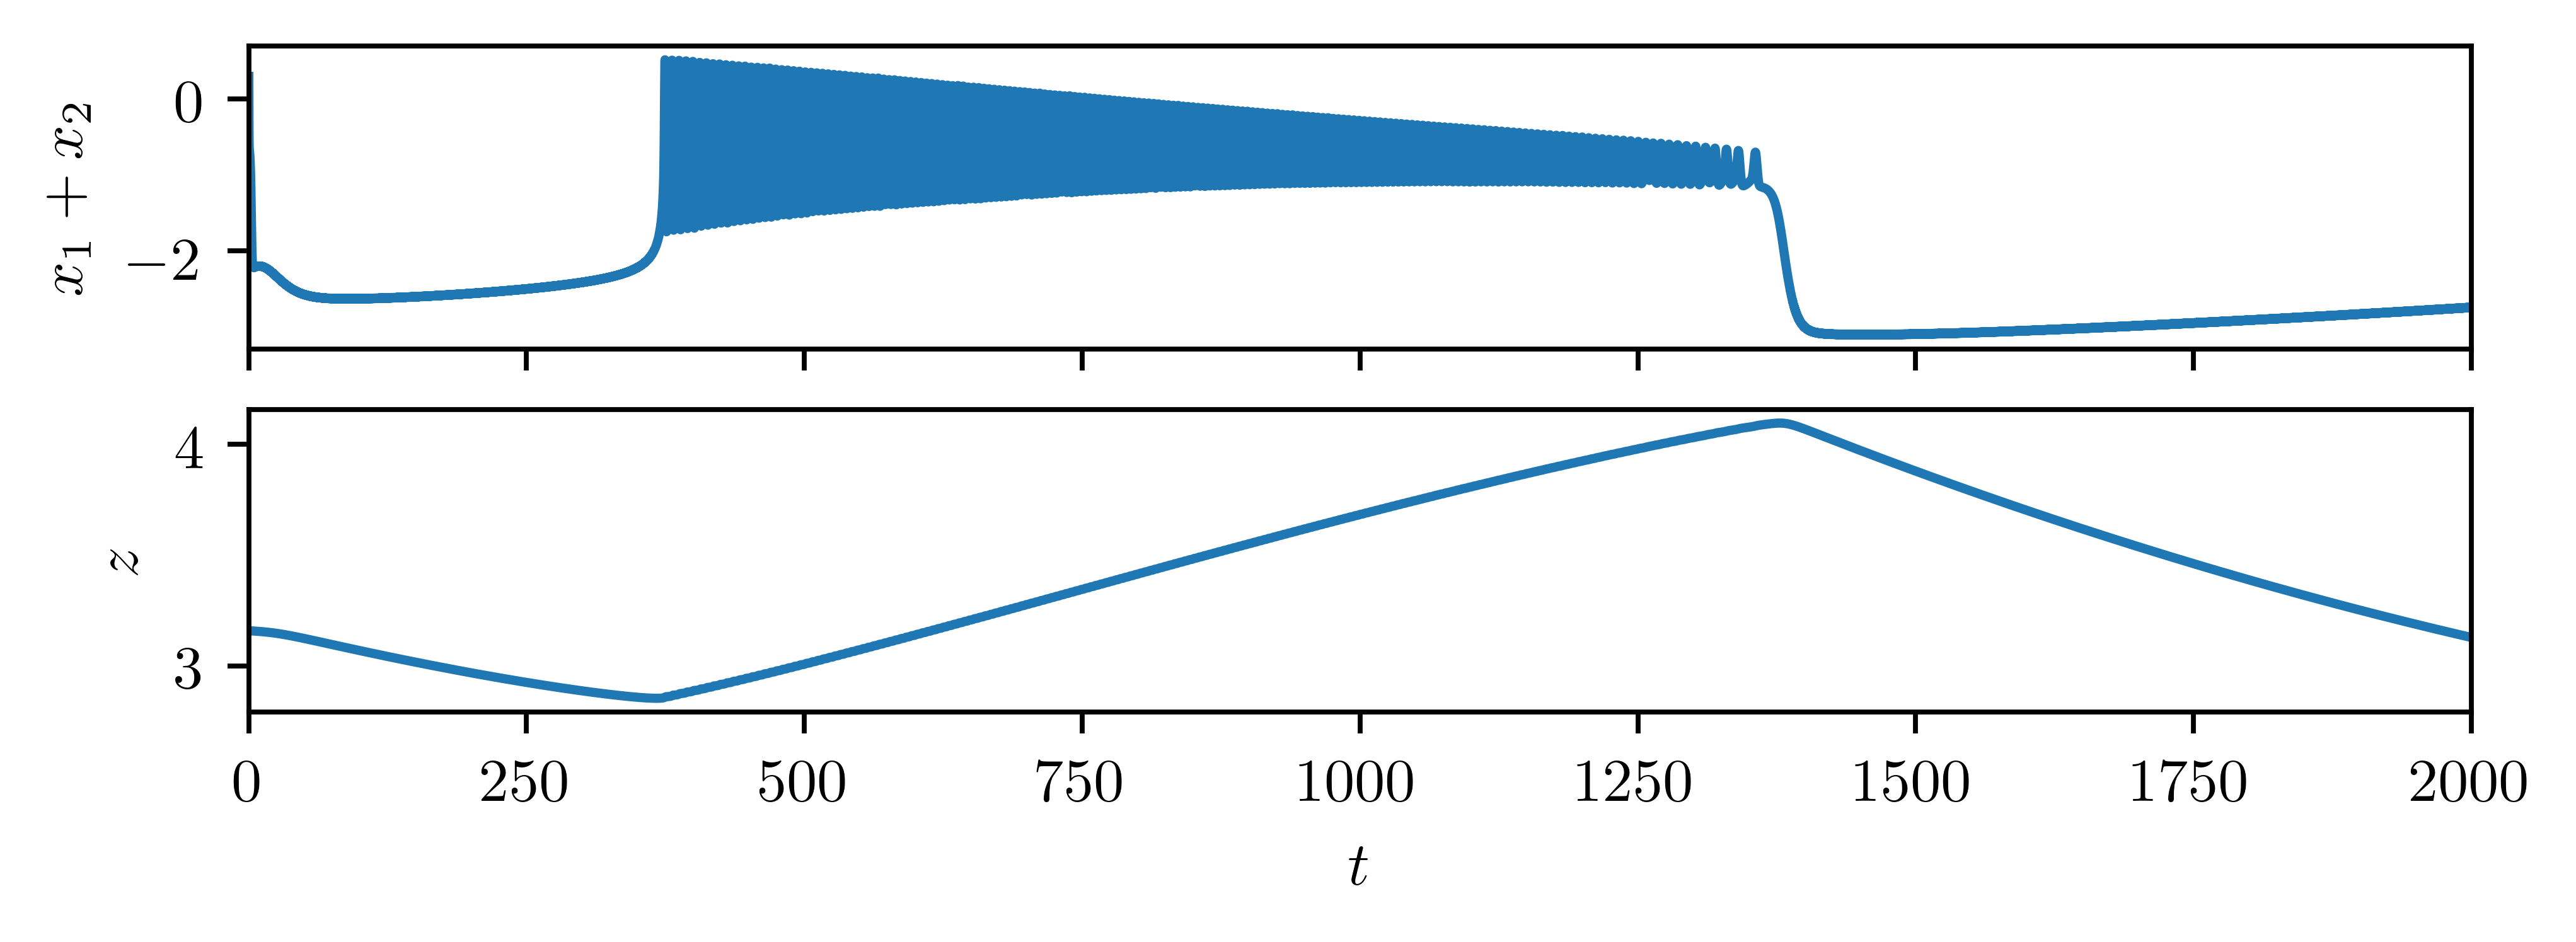
\includegraphics[width=\textwidth]{figure/epileptor}
    \caption{}
    \label{fig:epileptor}
  \end{subfigure} $\iff$
  \begin{subfigure}[c]{0.4\textwidth}
    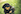
\includegraphics[width=\textwidth]{figure/midres}
    \caption{}
    \label{fig:midres}
  \end{subfigure}

  \begin{subfigure}[c]{0.4\textwidth}
    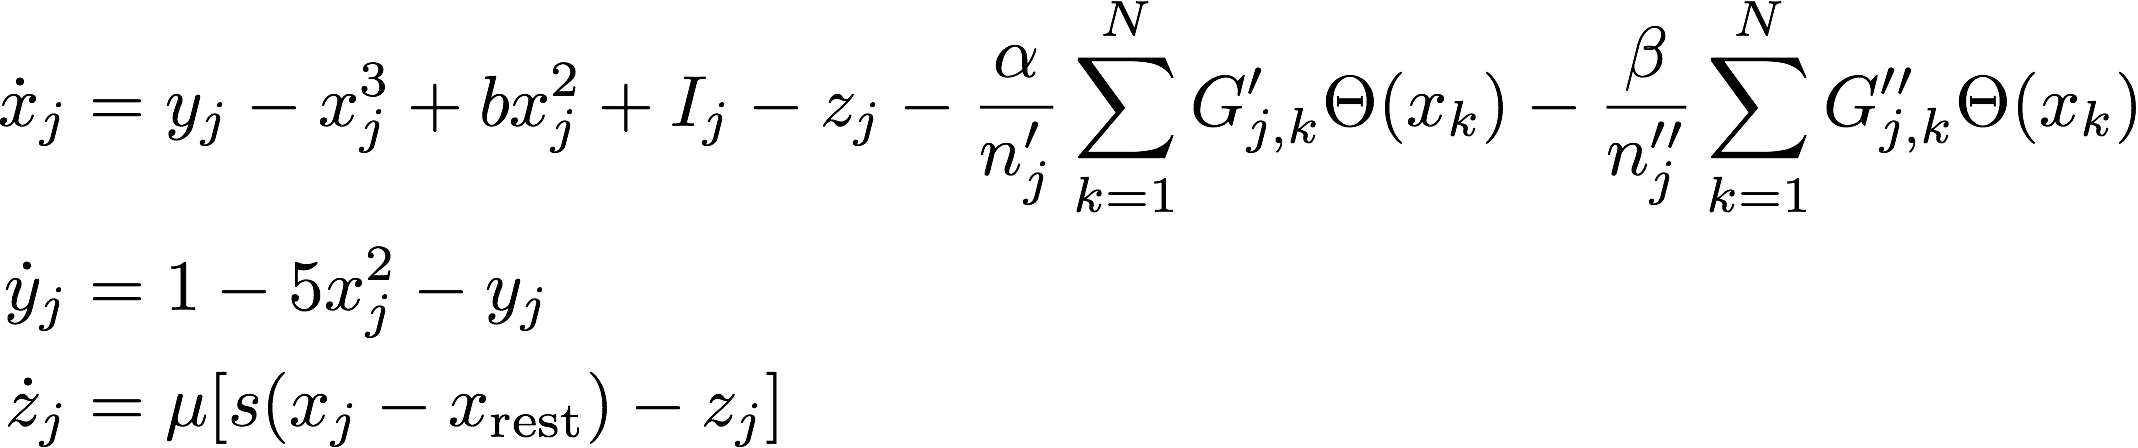
\includegraphics[width=\textwidth]{figure/HR}
    \caption{}
    \label{fig:HR}
  \end{subfigure} $\iff$
  \begin{subfigure}[c]{0.4\textwidth}
    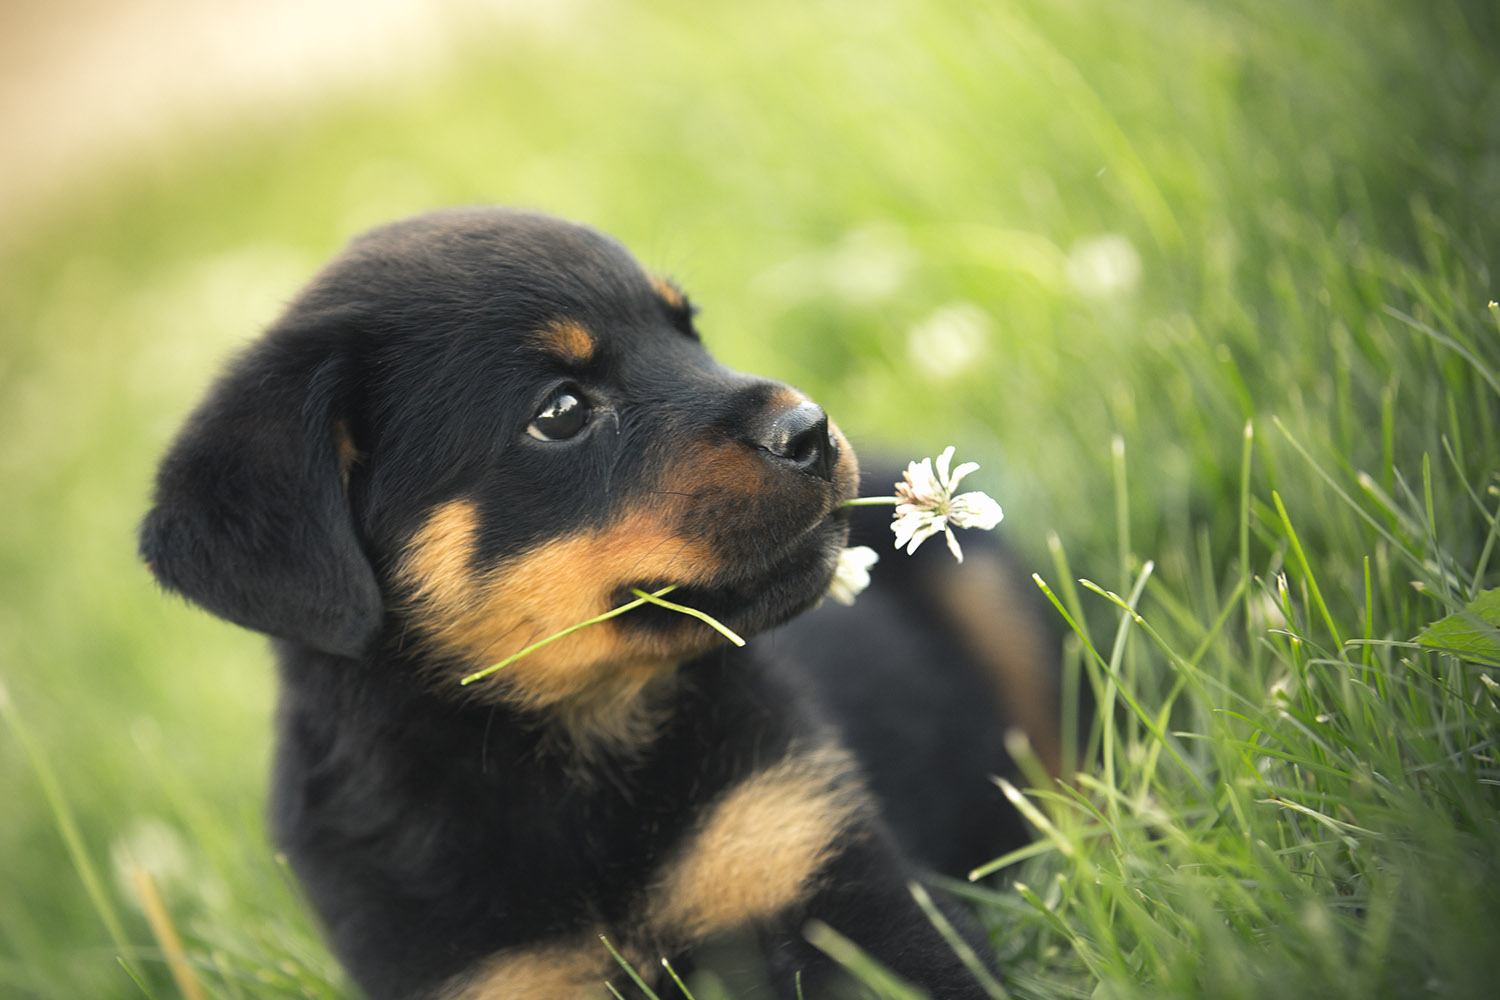
\includegraphics[width=\textwidth]{figure/puppy}
    \caption{}
    \label{fig:puppy}
  \end{subfigure}
  \caption{\Cref{fig:lumped} shows the model of Wang \etal, which gives a broad overview of brain activity.
  It reduces the extremely complex system of the brain to three dimensions, making it a relatively simple mathematical problem.
  However, much like describing the picture of the puppy as three RGB values (\cref{fig:bland}) sacrifices all spatial information and nuance from the photograph, using just three equations to describe the entire brain deprives us of a lot of knowledge of what is going on inside the various parts of the brain.
  \Cref{fig:epileptor} shows the Epileptor model, which describes the state of the brain as a whole.
  It takes into account the physical states of neurons around the brain, but still uses some simplifications that make it difficult to get an accurate picture of the state of the brain.
  This is like describing the puppy by giving information about a few key pixels, while still leaving a lot of information out.
  Finally, \cref{fig:HR} shows the HR model, which can be used at varying levels of precision.
  If we had perfect information about the connective structure of the brain, we could recreate its interactions perfectly using the HR model (\cref{fig:puppy}).
}
  \label{fig:analogy}
\end{figure}

The key alternative modeling technique is that of using a neuronal network \autocite{Lytton2008}.
This involves directly modeling networks of neurons.
As with any model, it comes with its benefits and downsides.
The two main downsides are first that an overly detailed model can negate the benefits that come from using an abstracting model in the first place, and the fact that detailed models require more computing power \autocite{Lytton2008}.
However, computing power improves exponentially with time, making larger-scale and more detailed models more useful as time goes on.

The benefits derived from these detailed models are noteworthy, as well.
As an example, a neuronal network model could describe the interactions between 65 different cortical areas via 1139 connections \autocite{Santos2017}.
The behavior of each area is described by the Hindmarsh-Rose (HR) neuron model, which is characterized by a set of coupled nonlinear differential equations.
These equations are not solvable analytically, but can be investigated numerically.
Additionally, each aspect of the equations corresponds to a measurable physical quantity.
Returning to the puppy analogy, these models give a wealth of information; instead of giving you a list of three numbers to describe the color of the whole picture, I could give you the RGB values for each pixel.
This would be overwhelming for you to deal with by yourself, but easy for a computer to convert into a perfectly clear picture of a puppy.
Similarly, the model is relatively easy to manage with sufficient computing power.

This specific model has exhibited some very interesting properties.
Chiefly, it has shown a propensity for chimera states, which are a deeply studied area in the world of nonlinear dynamics \autocite{Santos2017,Martens2013}.
Since chimera states have been observed for specific parameter values in this type of network, it would provide a good testing ground for analogies between epileptic seizures and collapses of chimera states into fully synchronous regimes \autocite{Andrzejak2016}.
The behavior of any model is supposed to directly mimic the behavior of the system it is modeling.
If the model exhibits a chimera state for a certain set of parameter values, then the brain should be in a chimera state for those same parameter values.
When the model shows a whole cortex of oscillating synchronously, while the rest of the brain oscillates asynchronously, the model is describing a focal seizure.
When this chimera state collapses into total synchrony, the model is describing secondary generalization of the seizure.
As the parameters of the model change over time (due to various chemical and environmental factors in the brain), the likelihood of chimera states (and therefore seizures) also changes.
However, given the recency of the publications making these claims, the comparisons have not been tested, and therefore provide a set of open questions for further exploration.

A model of an intermediate level of abstraction is commonly referred to as Epileptor \autocite{Jirsa2014}.
It lumps the brain into inhibitory and excitatory processes, operating at different time scales, but describes some of the behavior of these lumps using a physically-grounded model.
This model allows researchers to understand the system's behavior quite well, and use standard techniques of nonlinear dynamics in order to study its properties.
Its predictions match with data very well, but has some parameters which are not directly measurable, i.e., do not have a direct correspondence with a physiological state of a part of the brain.
This immeasurability makes Epileptor difficult to use as a real-time predictor of seizures, but does provide some insight into the mechanisms behind them.
For example, Epileptor's predictions include the phenomenon known as critical slowing-down \autocite{Jirsa2014}.
This means that, as a seizure approaches, any changes from the brain's normal baseline activity take much longer to return to normal.
This is a commonly observed phenomenon in many nonlinear systems, and Epileptor's predictions of its presence match with what has been observed \autocite{Scheffer2009}.

%%% Local Variables:
%%% mode: latex
%%% TeX-engine: xetex
%%% TeX-master: "../main"
%%% End:


\chapter{Methods}
\label{chap:methods}
%% The main analysis in this work is a modification of work by Santos et al.\ [\onlinecite{Santos2017}].
\subsection{Model}
\label{sec:methods_model}
The model used for this work was the modified Hindmarsh-Rose neural model\footnote{The modification is to add in the coupling, turning it into a network model instead of a single neuron.} \cite{Santos2017}.
\begin{align}
  \label{eq:hr_x}
  \dot{\hrx}_{j}
  &=
    \hry_{j}
    -
    \hrx_{j}^{3}
    +
    b \hrx_{j}^{2}
    +
    I_{j}
    -
    \hrz_{j}
    -
    \frac{\hra}{n'_{j}} \sum_{k = 1}^{N} G'_{j k} \Theta_{j}(\hrx_{k})
    -
    \frac{\hrb}{n''_{j}} \sum_{k = 1}^{N} G''_{j k} \Theta_{j}(\hrx_{k}) \\
  \label{eq:hr_y}
  \dot{\hry}_{j}
  &=
    1
    -
    5 \hrx_{j}^{2}
    -
    \hry_{j} \\
  \label{eq:hr_z}
  \dot{\hrz}_{j}
  &=
    \mu \pqty{s \pqty{\hrx_{j} - \hrx_{\text{rest}}} - \hrz_{j}}
\end{align}
where
\begin{equation}
  \label{eq:hr_sigmoid}
  \Theta_{j}(\hrx_{k})
  =
  \frac{\hrx_{j} - \hrx_{\text{rev}}}{1 + e^{-\lambda \pqty{\hrx_{k} - \theta}}}
\end{equation}
is the sigmoidal activation function, making it a neural mass model.
\Cref{tab:hr_params} shows the values and meanings of the symbols in the model.

\begin{table}[ht]
  \centering
  \begin{tabular}{c | c | l}
    Symbol & Value & Meaning \\ \hline
    $\hrx_{j}$ & --- & Membrane potential of the $j$th neural mass \\
    $\hry_{j}$ & --- & Associated with the fast processes \\
    $\hrz_{j}$ & --- & Associated with slow processes \\ \hline
    $b$ & 3.2 & Tunes the spiking frequency \\
    $I_{j}$ & 4.4 & External input current \\
    $\hrx_{\text{rev}}$ & 2 & Ambient reverse potential \\
    $\lambda$ & 10 & Sigmoidal activation function parameter \\
    $\theta$ & -0.25 & Sigmoidal activation function parameter \\
    $\mu$ & 0.01 & Time scale for variation of $z$ \\
    $s$ & 4 & Governs adaptation \\
    $\hrx_{\text{rest}}$ & -1.6 & Resting/equilibrium potential \\ \hline
    $\hra$ & Varied & Connection strength within cortices \\
    $n_{j}'$ & See \cref{fig:n_prime} & Number of connections within a cortex from the $j$th neuron \\
    $G_{j k}'$ & See \cref{fig:g_prime} & Intra-cortical connection matrix \\
    $\hrb$ & Varied & Connection strength between conrtices \\
    $n_{j}''$ & See \cref{fig:n_prime} & Number of connections between cortices from the $j$th neuron \\
    $G_{j k}''$ & See \cref{fig:g_prime} & Inter-cortical connection matrix
  \end{tabular}
  \caption[Hindmarsh-Rose Parameters]{The list of parameters used in modeling the Hindmarsh-Rose network.}
  \label{tab:hr_params}
\end{table}

This model was chosen due to the semanticity of its parameters, as well as its proven ability to exhibit chimera-like behavior as a neural mass model \cite{Santos2017}.
Additionally, the Hindmarsh-Rose model was not designed to emulate seizures, which provides further evidence for the theory that chimeras are a universal aspect of brain activity, as discussed in \cref{sec:lit_review_chimera_square_torus}.

%%% Local Variables:
%%% mode: latex
%%% TeX-master: "../../main"
%%% End:


\subsection{Network}
\label{sec:methods_network}
The model was implemented on a mesoscale mouse connectome, which organized the mouse brain into 213 fine areas, grouped into 13 coarse areas, and measured the connection strengths between the subcortices \cite{Oh2014}.
These coarse areas were used as the sets $C$ (\cref{eq:chimera,eq:metastability}) for chimera and metastability analyses.
The connection strengths were then reduced to those with sufficient certainty ($p < 0.01$), and segmented as follows:
\begin{equation}
  \label{eq:mouse_segmentation}
  G_{j k}
  =
  \begin{cases}
    0, & \text{if } O_{j k} < 10^{-4} \\
    1, & \text{if } 10^{-4} \leq O_{j k} < 10^{-2} \\
    2, & \text{if } 10^{-2} \leq O_{j k} < 1 \\
    3, & \text{if } 1 \leq O_{j k}
  \end{cases}
\end{equation}
where $O_{j k}$ is the raw connection strength provided by \cite{Oh2014}.
This was done to more closely match the analysis of Santos \textit{et al}.\ \cite{Santos2017}.

$G$ is shown in \cref{fig:mouse_connectome}, and is shown broken down into its inter- and intra-connections in \cref{fig:network_breakdown}.
A useful aspect of this brain network is that the standard graph whose topology it most resembles is a small-world or Watts-Strogatz graph \cite{Oh2014}.
This graph topology lends itself well to the development of chimera states, as it facilitates nonlocal coupling \cite{Hizanidis2016}.

\begin{figure}[ht]
  \centering
  \begin{subfigure}{0.45\textwidth}
    \centering
    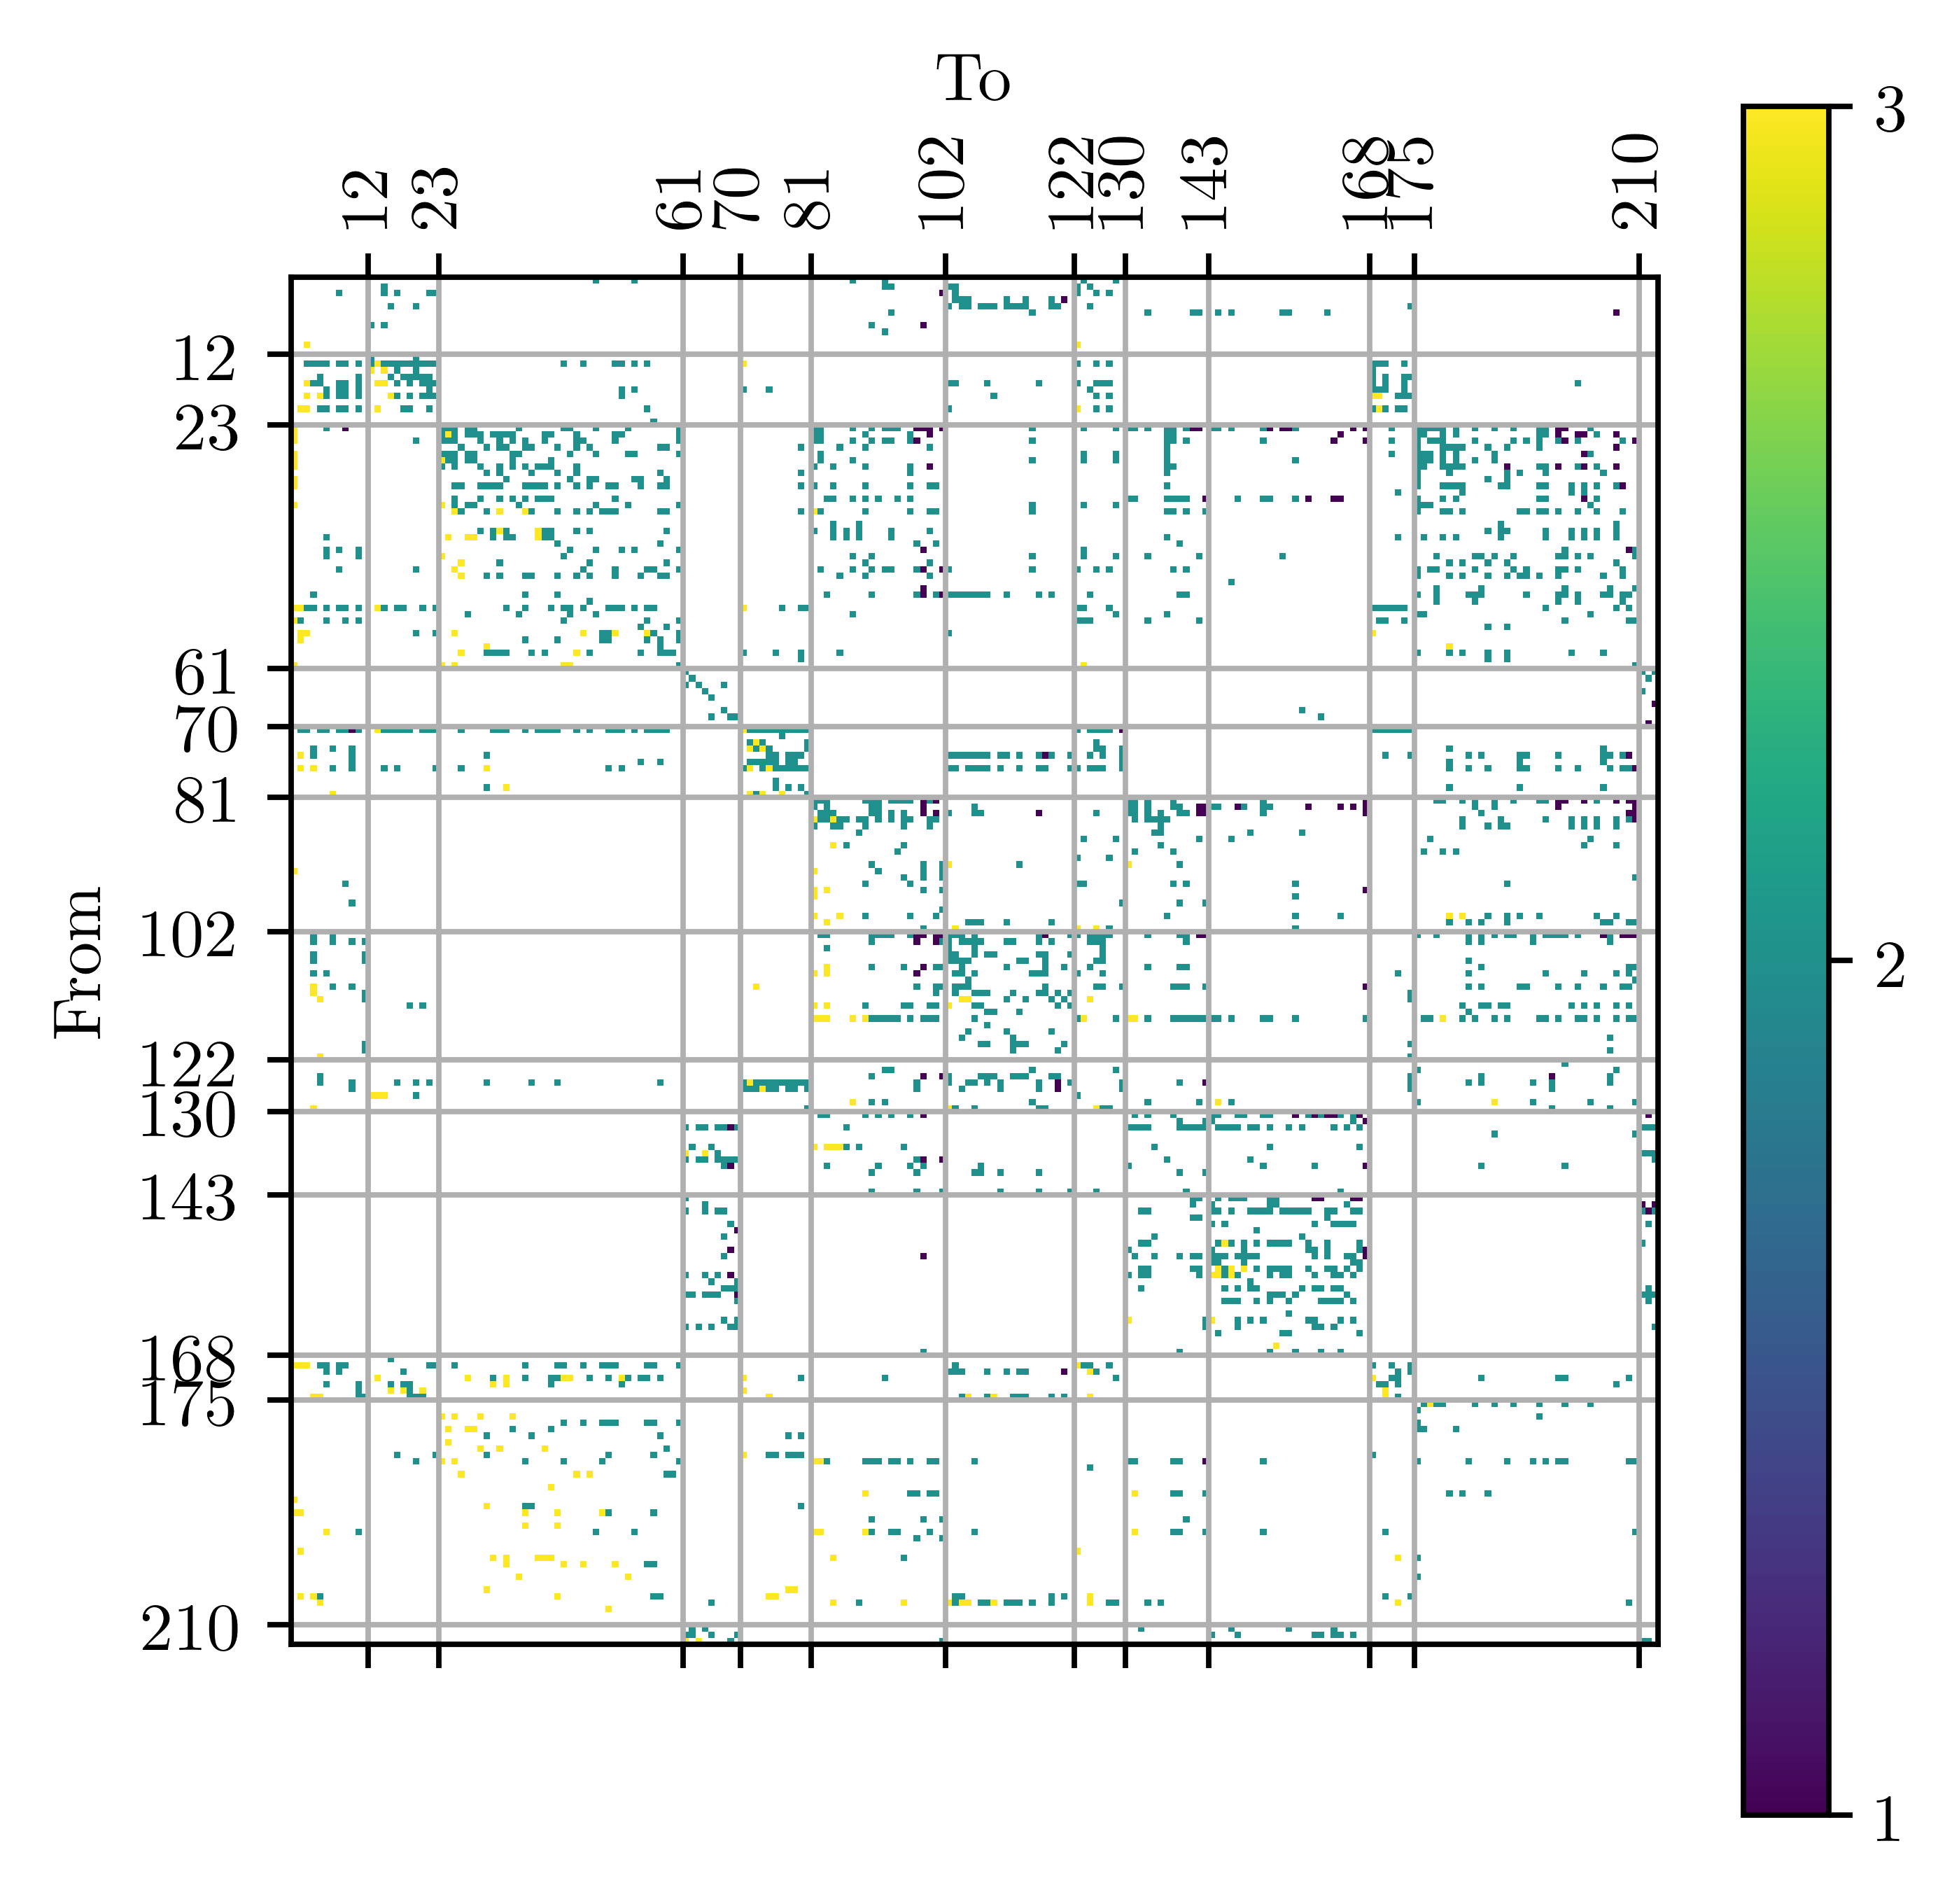
\includegraphics[width=\textwidth]{figure/n}
    \caption{Matrix representation}
    \label{fig:mouse_matrix}
  \end{subfigure} %
  \begin{subfigure}{0.45\textwidth}
    \centering
    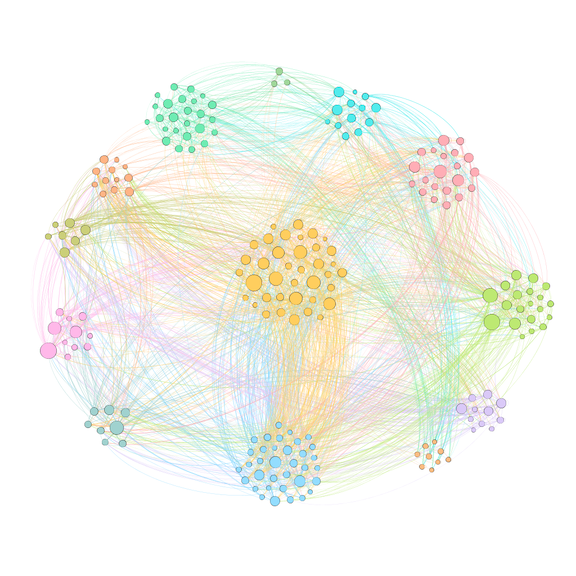
\includegraphics[width=\textwidth]{figure/network}
    \caption{Embedding}
    \label{fig:mouse_embedding}
  \end{subfigure}
  \caption[Mouse connectome]{(a) A matrix representation of the mouse connectome, with strengths as defined by \cref{eq:mouse_segmentation}.
    The cortices represented are, left to right (top to bottom),
    the striatum,
    the olfactory areas,
    the isocortex,
    the crebellar cortex,
    the hippocampal formation,
    the midbrain,
    the hypothalamus,
    the pallidum,
    the pons,
    the medulla,
    the cortical subplate,
    the thalamus,
    and the cerebellar nuclei.
    (b) An embedding of the graph.
    Edge colors indicate the source location.
  }
  \label{fig:mouse_connectome}
\end{figure}

Another benefit to this network is that it is accurate and complete.
Given the complexity of brains, creating an accurate structural or functional connectome is extremely difficult.
It has yet to be done to a large-scale extent in humans, and was only recently done in mice.
Additionally, as mice are common analogues for humans in laboratory settings, the mouse seemed a fitting ``guinea pig'' for the creation of chimera states.

\begin{figure}[ht]
  \centering
  \begin{subfigure}{0.45\textwidth}
    \centering
    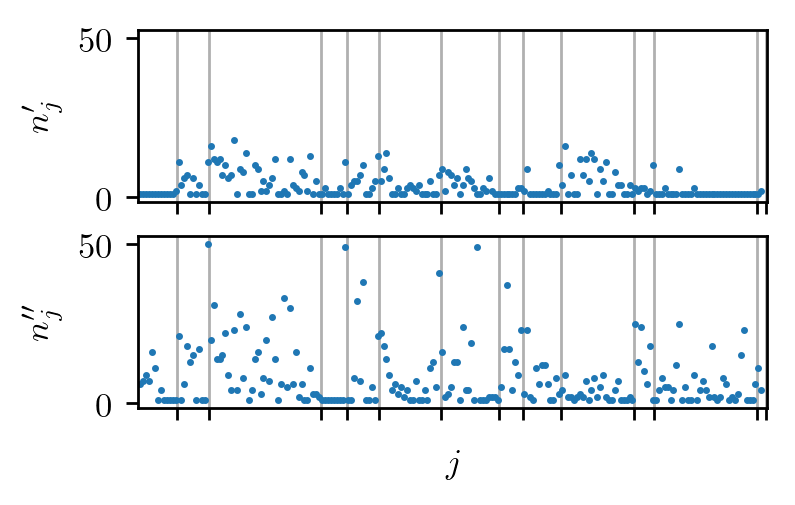
\includegraphics[width=\textwidth]{figure/n_prime}
    \caption{$n'$ and $n''$}
    \label{fig:n_prime}
  \end{subfigure} %
  \begin{subfigure}{0.45\textwidth}
    \centering
    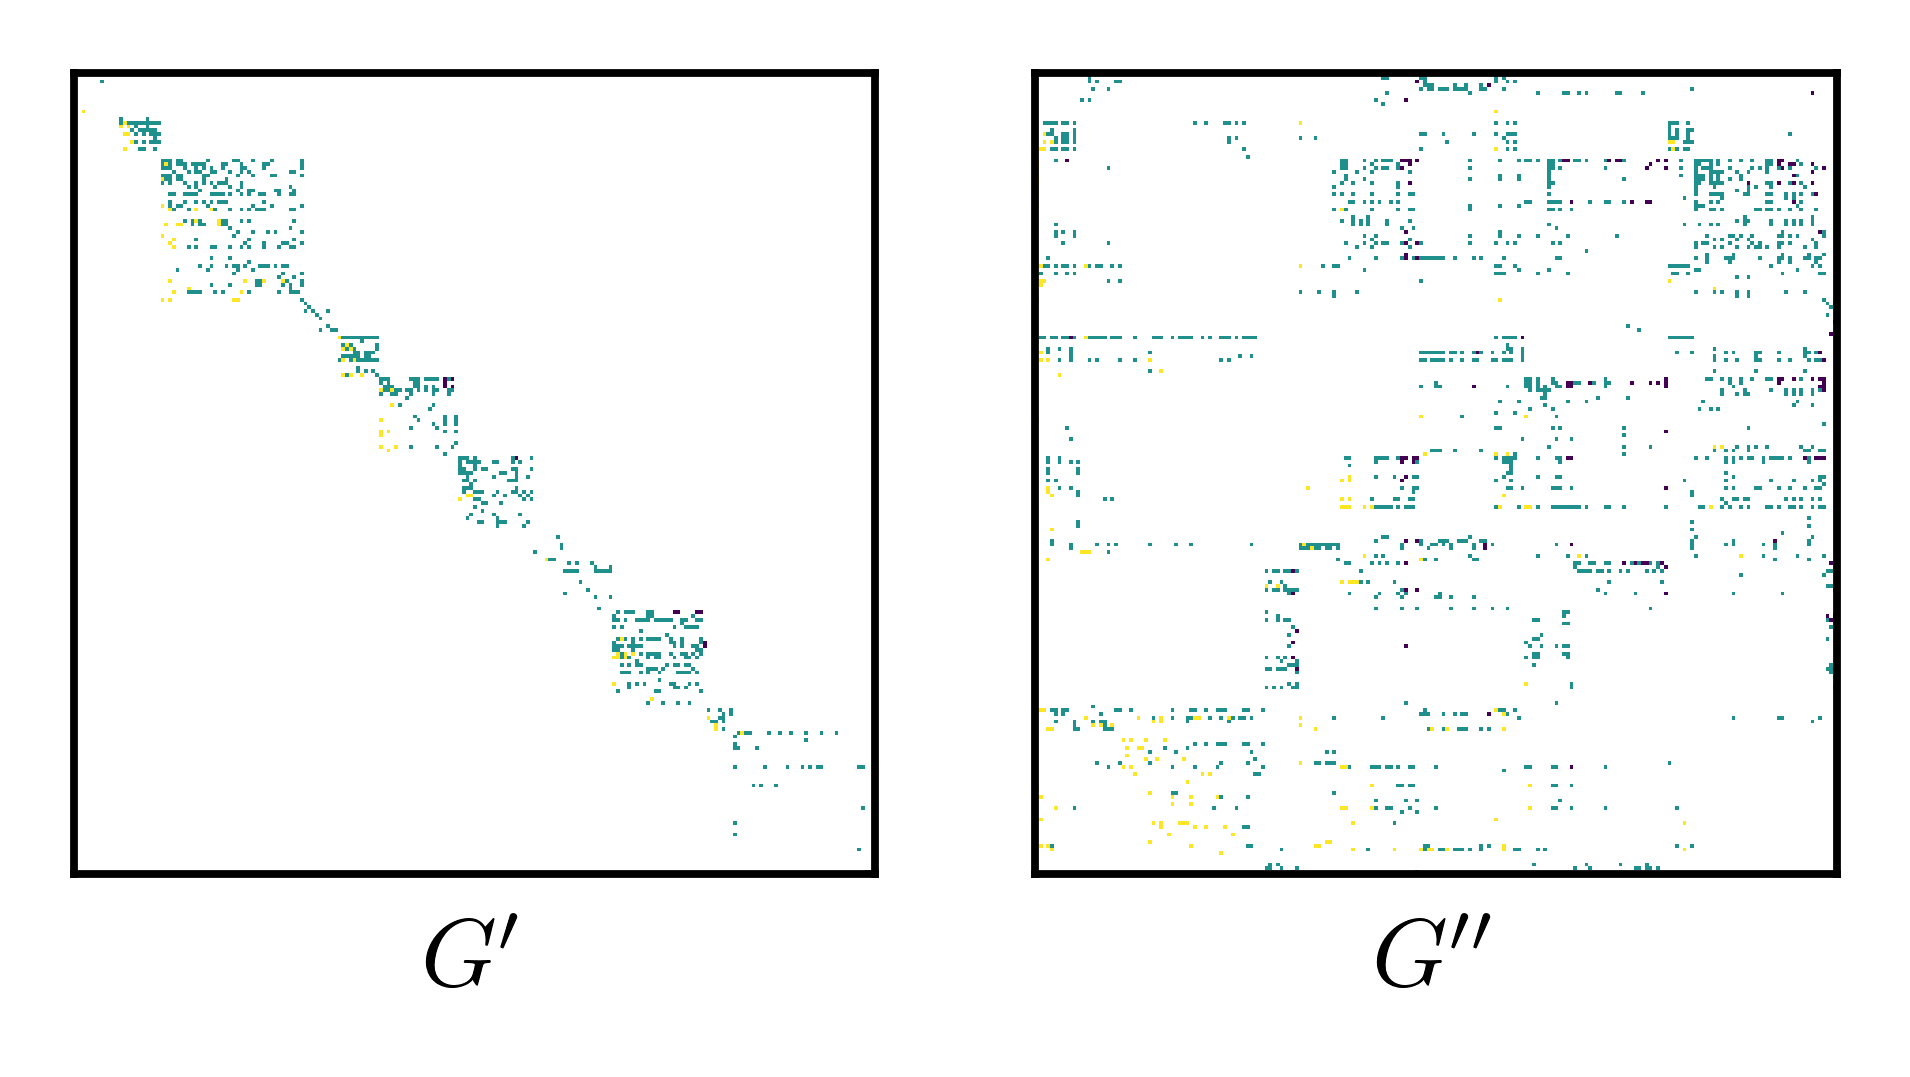
\includegraphics[width=\textwidth]{figure/g_prime}
    \caption{$G'$ and $G''$}
    \label{fig:g_prime}
  \end{subfigure}
  \caption[Network breakdown]{A breakdown of the network.
    (a) shows $n_{j}'$ and $n_{j}''$, effectively the number of nonzero elements in the $j$th row of $G'$ and $G''$, respectively.
    (b) shows $G'$ and $G''$, which are $G$ (\cref{fig:mouse_matrix}) only within and between cortices, respectively.
  }
  \label{fig:network_breakdown}
\end{figure}

\begin{figure}[ht]
  \centering
  \begin{subfigure}{0.45\textwidth}
    \centering
    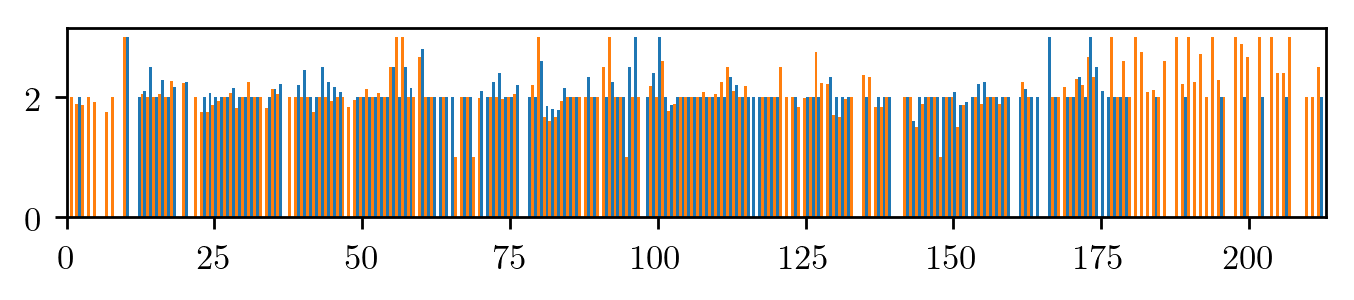
\includegraphics[width=\textwidth]{figure/g_over_n}
    \caption{All values}
    \label{fig:g_over_n}
  \end{subfigure} %
  \begin{subfigure}{0.45\textwidth}
    \centering
    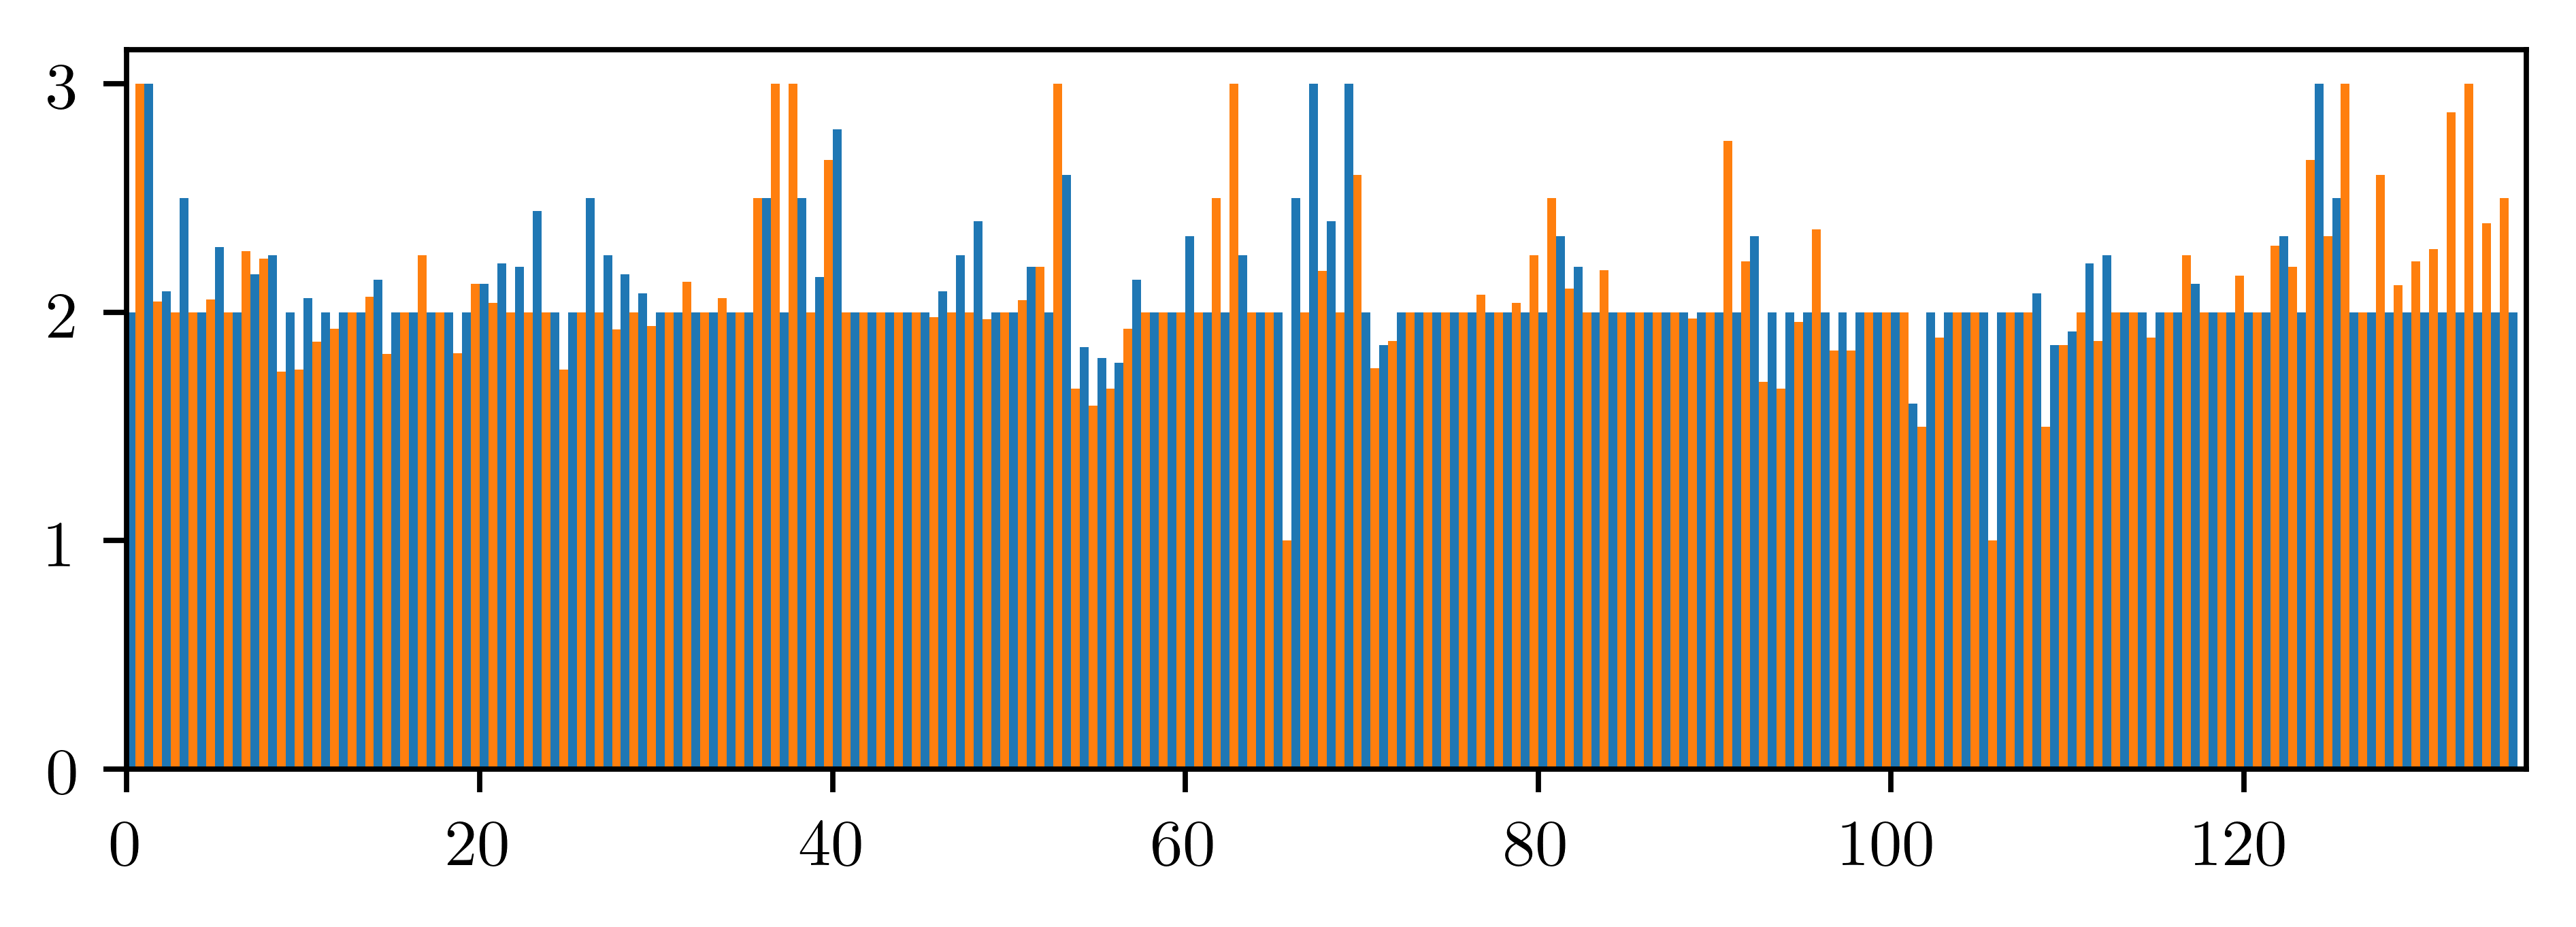
\includegraphics[width=\textwidth]{figure/g_over_n_drop}
    \caption{Dropped zeros}
    \label{fig:g_over_n_drop}
  \end{subfigure}
  \caption[Average strengths]{The average connection strengths for each neuron $j$, within cortices (blue) and between them (orange).
    (a) All of the subcortices.
    (b) All of the subcortices for which neither intra- nor inter-cortical average strength was 0.
  }
  \label{fig:average_strengths}
\end{figure}

%%% Local Variables:
%%% mode: latex
%%% TeX-master: "../../ms"
%%% End:


\subsection{Implementation}
\label{sec:methods_implementation}
The modified Hindmarsh-Rose model was coded into Python (Python version 3.7.0, NumPy version 1.15.2, Pandas version 0.23.4, SciPy version 1.1.0), and integrated using a 4th-order Runge-Kutta with variable step size\footnote{Step size was determined by SciPy's internal algorithms, but was limited to a maximum of 0.01.} $\dd{t} < 0.01$.
The code was verified by reproducing the results of \cite{Santos2017}.
The model was run for a time period of $T_{\text{sim}} = \bqty{-1000, 5000}$, where only times $T = \bqty{0, 4000}$ were saved.
The times $\bqty{-1000, 0}$ were calculated and thrown away to eliminate transients.
The chimeras were extremely unlikely to be eliminated on such a time scale, due to the size of the network \cite{Wolfrum2011}.
The times $\bqty{4000, 5000}$ were calculated to facilitate calculation of the phase.

The phase of the $j$th neuron in the resulting waveform was found as
\begin{equation}
  \label{eq:hr_phase}
  \phase_{j}(t)
  =
  2 \pi \times \frac{t - t_{k}}{t_{k + 1} - t_{k}}
\end{equation}
where $t_{k}$ is the time at which the $j$th neuron fires ($x_{j}$ crosses 0 in a positive direction) for the $k$th time.
In order for this calculation to be possible for all values in $T$, it was necessary to have each neuron fire at least once after $T$ had finished (i.e., there has to be some $t_{k + 1} \notin T$ in order to calculate the phase for times $t_{k} \leq t \leq t_{\text{max}} = 4000$).
The calculated time range went so far beyond $t_{\text{max}}$ so that any extremely slow-firing neurons were allowed to do so, to ensure that as much of parameter space was in the physical region (\cref{sec:results_aphysical}).
The phase was then used to find the chimera and metastability indices of the result using \cref{eq:chimera} and \cref{eq:metastability} respectively.

This process was repeated for various parameter sweeps of $\hra \times \hrb$, summarized in \cref{tab:parameter_sweeps}.
Note that the step in each strength $i \in \Bqty{\hra, \hrb}$ is $\Delta i = \frac{i_{\text{max}}}{n_{i} - 1}$, due to the fact that the ranges are inclusive of both endpoints.
\begin{table}[ht]
  \centering
  \begin{tabular}{c | c | c}
    $\hra_{\text{max}}$, $\hrb_{\text{max}}$ & $\Delta \hra$ ($n_{\hra}$), $\Delta \hrb$ ($n_{\hrb}$) & Figure \\ \hline
    1.6, 0.4 & 0.0203 (80), 0.0211 (20) & --- \\
    3.2, 0.8 & 0.0405 (80), 0.0205 (40) & --- \\
    0.2, 0.1 & 0.00253 (80), 0.00256 (40) & \cref{fig:zoom_chimera} \\
    0.9, 0.9 & 0.0101 (80), 0.0101 (80) & \cref{fig:aphysical_chimera}
  \end{tabular}
  \caption[Parameter sweeps]{The sweeps used in evaluating the effects of $\hra$ and $\hrb$ on the chimera and metastability indices.
    All parameter sweeps started at $(\hra, \hrb) = (0, 0)$.
  }
  \label{tab:parameter_sweeps}
\end{table}

Initial conditions were uniform distributions of $x_{j} \in \bqty{-2, 2}$, $y_{j} \in \bqty{0, 0.2}$, $z_{j} \in \bqty{0, 0.2}$.
All code was run on the \href{https://www.uvm.edu/vacc}{Vermont Advanced Computing Core}, and is \href{https://gitlab.uvm.edu/Henry.Mitchell/thesis}{available online}.

%%% Local Variables:
%%% mode: latex
%%% TeX-master: "../../main"
%%% End:


%%% Local Variables:
%%% mode: latex
%%% TeX-master: "../ms"
%%% End:


\chapter{Results}
\label{chap:results}
We now investigate three aspects of the results of this work.
First, we compare the output from the model to real-world data, on a qualitative level.
We then discuss the region of parameter space for which the model produces aphysical results.
Finally, we draw connections between chimera states in the model and their physiological analogues.
\section{Model Quality}
\label{sec:results_model}


\section{Aphysical Region}
\label{sec:results_aphysical}


\section{Chimera states}
\label{sec:results_chimera}


\chapter{Conclusion}
\label{chap:conclusion}
\section{Future Work}
\label{sec:conclusion_future_work}
The logical next step is to compare the simulated EEG traces to actual data collected from mice, with the aid of an epileptologist.
With further work in this direction, our research could potentially go from a mathematical curiosity to an applicable therapeutic and diagnostic tool.

Finding an instructive phase-space embedding of the Hindmarsh-Rose network would be challenging (seeing as it is a 639-dimensional system),
but would likely reveal potentially useful insights into the nature of the mechanisms underlying these systems.
The same could be said for Lyapunov analysis, as well as finding an informative way to create a bifurcation diagram and perform more in-depth bifurcation analysis.

Another way our work could be extended is by looking at chimera state collapse and its relationship to secondary seizure generalization.
However, it would be extremely computationally expensive, given the size of the system, and would therefore require some clever handiwork [\onlinecite{Wolfrum2011}].

Future work could also naturally be performed on better, more up-to-date connectomes [\onlinecite{Knox2019}].

%%% Local Variables:
%%% mode: latex
%%% TeX-master: "../../ms"
%%% End:


\section{Acknowledgments}
\label{sec:conclusion_acknowledgements}
This work could not have been completed without help from Taras Lakoba and Sean Flynn.
The authors also thank Kameron Harris for helpful comments on the manuscript.


\appendix

\listoffigures

\listoftables

\printbibliography

\end{document}


%%% Local Variables:
%%% mode: latex
%%% TeX-master: t
%%% End:
